\BiChapter{卷积神经网络}{CNN}
卷积神经网络灵感源自哺乳动物的视觉系统,它是唯一一个不需要预训练便能直接训练的深度网络。LeCun在1989年设计了第一个卷积神经网络,并将这个网络运用到邮编数字识别中取得了很好的效果,随后,xxxx将卷积神经网络应用到文档识别中,实现了可理解数字串的网络,这是一个重大的突破。但卷积神经网络在提出的二十多年里一直默默无闻,直到最近几年,人们发现在图像识别中卷积神经网络相比于其他的模型能更好地进行特征提取才被重视。目前,几乎所有最好的识别系统都是基于卷积神经网络的,从某种意义上而言,卷积神经网络相当于深度学习的代言人。
\BiSection{卷积神经网络综述}
x卷积神经网络可以看做是一种特殊的神经网络,在深度置信网络中,网络节点是全连接的,而卷积神经网络中连接是局部的。此外,卷积网络强制权值共享,对比于深度置信网络,卷积网络的这些特性都体现着非常强的正则。

\begin{figure}[htbp]
\centering
\subfigure{\label{img:fullNN2D}}\addtocounter{subfigure}{-2}
\subfigure{\subfigure[全连接神经网络]
			{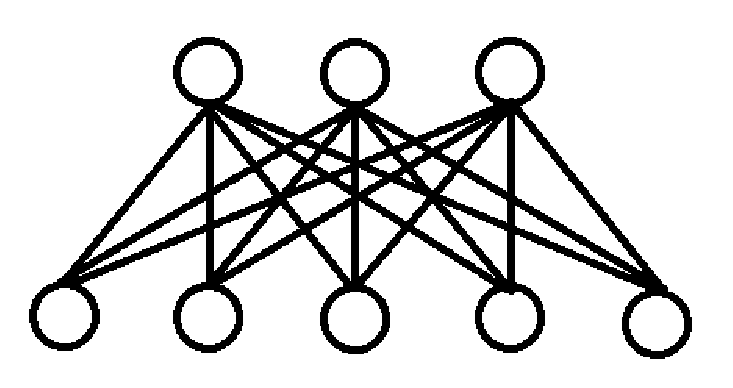
\includegraphics[width=0.4\textwidth]{CNN/fullNN2d.eps}}}
\subfigure{\label{img:conv2D}}\addtocounter{subfigure}{-2}
\subfigure{\subfigure[卷积神经网络]
			{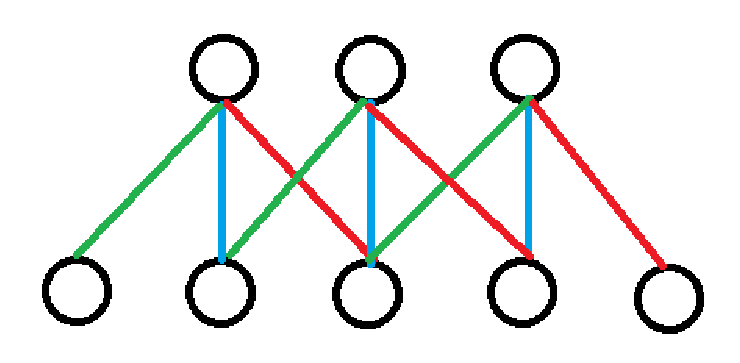
\includegraphics[width=0.4\textwidth]{CNN/convNN2d.eps}}}
\caption{二维视觉下的全连接神经网络与卷积神经网络}
\vspace{-1em}
\end{figure}

如图\ref{img:fullNN2D}所示为传统的全连接神经网络,我们可以看到,每一个上层节点与下层节点都含有连接,而所有的连接都是独立无关联的,即每个连接权值都不相等。对应的,图\ref{img:conv2D}所示为卷积神经网络,在这种网络构型中,每个上层节点只与部分的下层节点连接,并且,这些连接的权值是共享的,即相同颜色的连接代表其权值相等。局部连接将会大大减少网络的连接数量,而权值共享又会大大减少网络的参数数量。例如在图\ref{img:conv2D}中,连接数量为$3\times 5 = 15$,由于权值不共享,其参数数量也是15。而图\ref{img:conv2D}的连接数量为$3\times 3$,权值共享使得网络的参数只有3个。卷积网络的设计目的是让网络拥有更多的连接,而拥有更少的权值。尽管这里连接数量上卷积网络要比全连接网络少,但是我们后面将会看到,卷积网络将通过多张特征图构造出更多的连接。

卷积神经网络,一般用于图像识别与声音识别两个领域,因为这两个领域带着明显的二维特性。例如在图像识别中,图像即可以看做是高维的,也可以看做是二维的,如果将它看做高维的,那么就是将像素点展开成为一个高维列向量,展开后的图像将不再具有原始的面貌。如果将它看做是二维的,就是保留图像的原貌,利用二维的平面直角坐标系来描述。声音之所以可以看做二维的,是因为它带有时间这一维度,关于声音识别,我们不过多讨论,更多的细节请参考文献xxxx。

\begin{figure}[htbp]
\centering
\subfigure{\label{img:fullNN3D}}\addtocounter{subfigure}{-2}
\subfigure{\subfigure[全连接神经网络]
			{\includegraphics[width=0.4\textwidth]{CNN/fullNN3d.eps}}}
\subfigure{\label{img:convNN3D}}\addtocounter{subfigure}{-2}
\subfigure{\subfigure[卷积神经网络]
			{\includegraphics[width=0.4\textwidth]{CNN/convNN3d.eps}}}
\caption{三维视觉下的全连接神经网络与卷积神经网络}
\vspace{-1em}
\end{figure}

由于卷积网络保留了图像的二维面貌,因此相比于全连接神经网络而言,其网络构型是一个三维构型,如图\ref{img:fullNN3D}所示为三维视觉下全连接神经网络。由于上层节点是一个高维列向量,我们可以认为这个向量是一维的,并且这个向量里的每一个元素都与输入图像上的每一个像素点连接,不同元素之间的连接权值是不同的。而图\ref{img:convNN3D}所示是三维视觉下的卷积神经网络,我们可以看到,上层节点是一个二维矩阵,因此它的特征我们可以认为是二维的,这些上层节点组成的二维矩阵我们称为特征图(feature map),特征图里的每一个元素,都只与输入图像上的一小块区域有连接,并且,特征图里的不同元素的连接权值是相等,这些相同的连接权值我们称之为卷积核(convlution kernel)。图\ref{img:convNN3D}仅仅是一张特征图,实际中的卷积神经网络,往往通过多个不同的卷积核,卷积出多张特征图。

\BiSection{卷积神经网络的前馈}
x一个完整的卷积神经网络应包含三个内容:卷积层、采样层以及全连接层,关于各层的细节以及作用我们将在后面的小节中叙述,现在让我们先大致了解卷积神经网络的结构。如图\ref{img:CNN}所示是卷积神经网络其网络构型
\begin{figure}[!htbp]
\centering
\includegraphics[width=0.8\textwidth]{CNN/CNN.eps}
\caption{卷积神经网络网络构型}
\label{img:CNN}
\end{figure}

在这种结构中,卷积层与采样层交错出现,在网络顶端采用全连接神经网络或其他分类器。图中卷积层里的每一张特征图,其执行过程都如图\ref{img:convNN3D}所示,这些不同的特征图对应着不同的卷积核,多张特征图,增加了网络的连接数目,但由于每张特征图只对应一个卷积核,所以网络的参数(即卷积核)的数目相比与全连接神经网络参数的数目而言是很小的。

\BiSubsection{卷积}
x卷积神经网络所使用的卷积即二维离散卷积,其定义为
\begin{equation}
\begin{split}
y[s, t] &= \sum\limits_{i=1}^{m_1 +  m_2 -1}\sum \limits_{j=1}^{n_1 + n_2 -1} x[i, j]\cdot k[s-i+1, t-j+1]\\
&~~~~~~~ 1\leq s \leq m_1 + m_2 -1\\
&~~~~~~~ 1\leq t  \leq n_1  + n_2 - 1
\end{split}
\end{equation}

式中,$x$为$m_1\times n_1$的矩阵,称为原始数据,$x[i,j]$代表$x$中的第$i$行第$j$列元素。$k$为$m_2 \times n_2$的矩阵,称为卷积核,$k[i, j]$代表$k$中的第$i$行第$j$列元素。$y$为$(m_1 + m_2 -1)\times (n_1 + n_2 -1)$的矩阵,称为卷积结果,$y[i, j]$代表$y$中的第$i$行第$j$列元素。如果从图像上来解释二维离散卷积,卷积层的操作相当于图\ref{img:convlution}所描述的过程。图中,原始图像是一张$5\times 5$像素的数字“4”的二值图像,如果我们定义卷积核为
\begin{equation}
kernel = \left[
\begin{array}{ccc}
~0~&~~~0~~~&~0~\\
~0~&~~~2~~~&~0~\\
~0~&~~~0~~~&~0~
\end{array}
\right]\label{equ:kernel}
\end{equation}

\begin{figure}[!htbp]
\centering
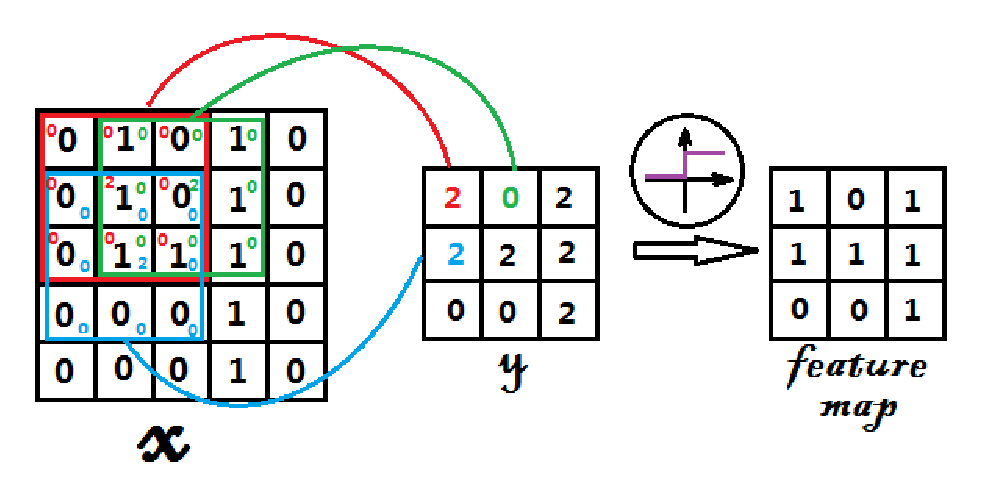
\includegraphics[width=0.8\textwidth]{CNN/convlution.eps}
\caption{卷积神经网络网络构型}
\label{img:convlution}
\end{figure}

那么经过二维离散卷积后,其得到的卷积结果为
\begin{equation}
y = x * kernel = 
\left[
\begin{array}{ccc}
~2~&~~~0~~~&~2~\\
~2~&~~~2~~~&~2~\\
~0~&~~~0~~~&~2~
\end{array}
\right]
\end{equation}
将卷积结果再经过一个阶跃函数进行非线性变换后,我们可以看到,卷积层通过式\eqref{equ:kernel}中定义的卷积核对原始图像(即数字4)进行卷积后,其非线性化后的结果依然保留着数字4的特征。由于卷积核是固定的,因此卷积操作经常被认为是一种滤波,即用卷积核去检测特征,将这些特征提取出来。

图\ref{img:convlution}只是利用一个卷积核对原始图片进行卷积得到一张特征图,事实上,正如图\ref{img:CNN}所示,如果我们利用多个卷积核对原始图像进行卷积,那么便可以得到多张特征图。多张特征图,意味着可以提取到原始图像的多个特征,例如在手写数字识别中,我们提取了三张特征图,其中一张特征图表明左上角有一点,一张特征图表明右上角有一个折线,剩下的一张特征图表明右下角有一个点,那么通过这三张特征图,我们就可以判定这个数字是“7”。特征图的作用,在于降低数据的冗余信息,例如“7”这个数字中,横线事实上只需要两个点就可以确定一条直线,竖线也同理只需要两点便可确定一条直线,然而横线与竖线之间存在一个相对位移,因此折线的作用便是刻画相对位移的。

图\ref{img:convlution}中的例子只针对与原始输入数据是一张图像的情况,实际上,卷积操作应该泛化到输入图像为多张的情况。例如,图图\ref{img:CNN}中的第二个卷积层,其输入图像便是多张图像。实际中,输入图像也不太可能是一张图像,一张输入图像的情况往往只出现于灰度图像中。然而在彩色图像中,我们知道,彩色图像是具有三张矩阵的,分别代表红(R)、绿(G)、蓝(B)。对于输入图像为多张的情况,解决的方法有两种。一种是利用同一个卷积核去卷积所有的$n$输入图像,将得到的$n$张卷积结果进行相加合并成为一张,在将它进行非线性映射,从而得到一张特征图,这个过程如图\ref{img:convlution4featuremap}所示。

\begin{figure}[!htbp]
\centering
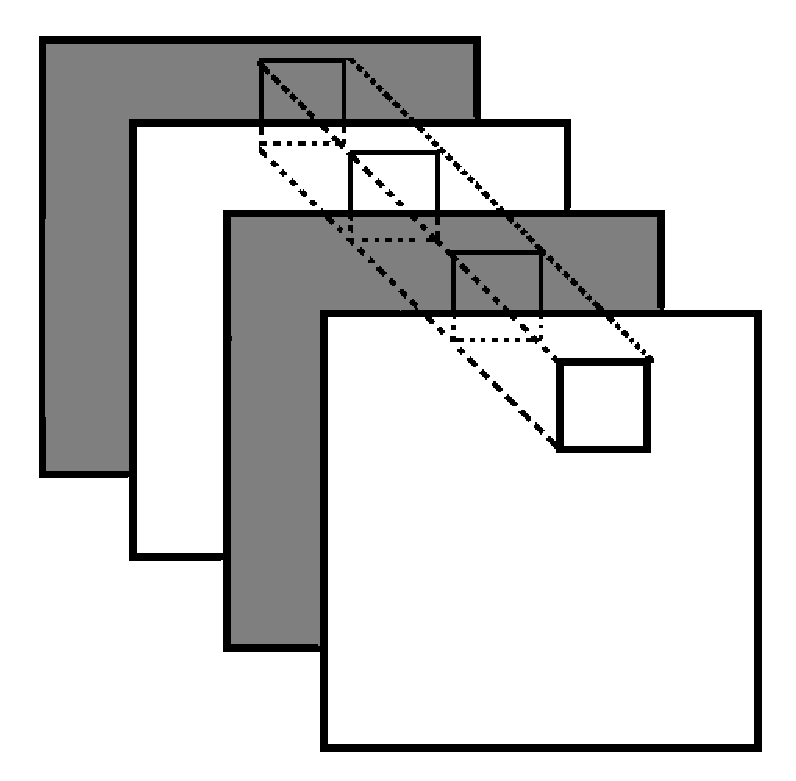
\includegraphics[width=0.3\textwidth]{CNN/convlution4featuremap.eps}
\caption{使用同一卷积核卷积多张图像}
\label{img:convlution4featuremap}
\end{figure}

另外一种解决方法是,假设我们有$ m $张输入特征图,而我们想要卷积后得到$ n $ 张输出特征图,那么我们使用 $m \times n$ 个卷积核,令$ k_{i,j}$ 代表从第$ i $张输入特征图映射到第$ j $张输出特征图这个过程中所需要使用的卷积核,$ b_j $代表卷积完成后第$  j $张特征图所要加上的偏置,那么卷积操作就可以描述为:
\begin{equation}
\bigg[\mathcal{M}_1, \mathcal{M}_2, \cdots, \mathcal{M}_m\bigg] \divideontimes \left[
\begin{array}{cccc}
k_{1,1} & k_{1, 2}, & \cdots, & k_{1, n} \\
k_{2,1} & k_{2, 2}, & \cdots, & k_{2, n} \\
\vdots &\vdots & \ddots  & \vdots \\
k_{m,1} & k_{m, 2}, & \cdots, & k_{m, n} \\
\end{array}
\right ] \boxplus \bigg[b_1, b_2, \cdots, b_n\bigg] = \bigg[\mathbf{M}_1,\mathbf{M}_2, \cdots, \mathbf{M}_n\bigg]
\label{equ:muticonv}
\end{equation}
式中,$\big\{\mathcal{M}_i\big\}_{i=1}^m$为$m$张输入特征图,$\big\{\mathbf{M}_j\big\}_{j=1}^n$为$ n $张输出卷积结果, $\boxplus$为面向元素的加法,$\divideontimes $是我们提出的一种运算,其运算与矩阵乘法类似,唯一不同是在元素操作时,矩阵乘法执行的是乘法操作, 而$\divideontimes $执行的是卷积操作。卷积操作完成后,再进行非线性映射,即可得到多张特征图。式\eqref{equ:muticonv}实际上类似于全连接神经网络的前向传播,但是不同的是,全连接神经网络中,$m \times n$矩阵里的每一个元素代表连接权值,是一个常数,而式\eqref{equ:muticonv}中,$m \times n$矩阵里的每一个元素代表一个卷积核,是一个矩阵。另外一个不同点在于,全连接神经网络执行的是乘法,而式\eqref{equ:muticonv}中执行的是卷积。

事实上,第一种解决方案只是第二中解决方案的特例,在第一种解决方案中,实际上相当于$K_{m \times n}$中的每一列都强制相等,即
\begin{equation}
k_{1, 1} = k_{2, 1} = \cdots = k_{m, 1}
\end{equation}
因此,第一种解决方案意味着更强的正则,或者说更强的惩罚,因为它强制每一列的卷积核都相等。但是我个人认为,尽管这种方法确实能工作得很好,但这是不太合理的。例如在图像中,三个输入图像,也就是RGB三个矩阵,采用第一种方案意味着对三个颜色都同等对待,因为作用在三个矩阵上的卷积核是相同的。但我们直觉上可以感觉到,这三种颜色不应该同等对待,而应区分开来,因此在往后的讨论中,我们只讨论第二种解决方案。

\BiSubsection{采样}
x卷积得到的特征图,需要经过一个采样层,采样层是针对每一张特征图的,即各张特征图的采样时独立互不干扰的,因此采样得到的特征图与原始的特征图之间是一一对应关系。假设我们使用一个均值采样,对于一个$4\times 4$的特征图,我们对其每$2\times 2$区域内取平均,即

\begin{equation}
\left[
\begin{array}{cccc}
1 &~~~~1 &~~~~2& ~~~~2\\
1 &~~~~1 &~~~~2& ~~~~2\\
3 &~~~~3 &~~~~4 &~~~~4\\
3 &~~~~3 &~~~~4 &~~~~4\\
\end{array}
\right] \rightarrow \left[
\begin{array}{cc}
1&~~2\\
3&~~4\\
\end{array}
\right]
\end{equation}

采样层的作用在于压缩数据,使得维度不至于快速增长。想象一个原本为$6\times 6$像素的原始图片,在经过一个$3\times 3$的卷积核进行卷积后,得到的特征图大小为$4\times 4$,但这只是一张特征图,由于在卷积层中我们往往使用多个卷积核进行卷积,假设我们设定卷积层的输出特征图总量为50,那么将会有$50\times 4 \times 4 = 800$个节点,而原来的节点只有$5\times 5 = 25$个节点,这将会使节点增加了32倍。采样层一般都是对卷积得到的特征图进行2倍的缩小,仅此经过采样层后,特征图的大小为$2\times 2$,此时的节点仅为$50\times 2 \times 2 = 200$个。

另一方面,采样层可以抑制位移的变化,卷积得到的特征图,在经过小区域内的平均后,弱化了其绝对位置,而保留了其相对位置,需要注意的是,这里的位移并不仅仅只欧式距离里的位移,还应包括图像的伸缩,旋转等,所以这个位移应理解为广义的位移。

采样的方法除了上面提到的平均采样方案,还有一些别的方案,例如xxx文献中介绍了一种自学习的采样,即小区域内并不是简单的求和取平均,而是类似于加权求和取平均,这些权值便是所需要学习的参数。这两种方案并没有孰劣孰优的说法,实际上两者都能很好的工作,但自学习的方法确实是会比简单的平均采样好一些,但由于平均采样更简单,所以我们往后的讨论只使用平均采样。

\BiSubsection{分类器}
x原始输入数据经过多次卷积采样后,特征图的尺寸不断缩小,最后将使得卷积无法再进行,此时,我们将这些非常小的特征图展开成为一个列向量。例如,一个原始图片为$32\times 32$大小的图像,经过一个$5\times 5$大小的卷积核后得到$28\times 28$的特征图,对其进行均值采样,将变为$14\times 14$大小的特征图,再用$5\times 5$大小的卷积核卷积,将得到$10\times 10$大小的特征图,采样后为$5\times 5$大小,此时再执行一次卷积后,特征图大小为$1\times 1$,这时候再也无法进行采样了,假设现在有100个$1\times 1$大小的特征图,那么它便可以展开成为一个100维的列向量。又例如,一个原始图片为$28\times 28$大小的图像,如果卷积核都设定为$5\times 5$,那么经过卷积、采样、卷积、采样后,将得到$4\times 4$的特征图,此时卷积核尺寸大于特征图的尺寸,卷积无法执行,应将这些特征图展开,假设有10张$4\times 4$的特征图,那么展开后将得到$10 \times 4 \times 4 = 160$维的列向量。

对于最后的列向量,即可以直接使用分类器,也可以在这些列向量的基础上搭建几层隐含层后再使用分类器,这个分类器可以是全连接神经网络或支撑向量机等,选取哪个取决于设计者的意愿。关于分类器如何使用,读者可以参考前面的章节,在卷积网络最顶层的分类器中,与传统神经网络是相同的。

\BiSection{卷积神经网络的反馈}
x卷积神经网络的训练方法与传统神经网络的训练方法类似,都是采用反向传播算法,但由于卷积网络特殊的构型,需要对其进行一些改动,但两者的核心都是相同的,即通过后一层的误差注入前一层中,乘上该层激活函数相对于净激活的偏导数后得到该层的误差,利用这个误差乘上净激活相对于输入的偏导数即可得到参数更新的增量。唯一的不同点在于注入的方式不同。
\BiSubsection{分类器误差传播}
x由于卷积神经网络中最顶层与传统的神经网络相同,因此参数校正以及反向传播方式是相同的。有一点需要注意的是,如果网络最后一个卷积层(或采样层)中将特征图拉成一个列向量,那么反向传播的时候需要将列向量还原回特征图形式,例如,如果网络中最后阶段得到10张$4\times 4$大小的特征图,前向传播过程中会将它们合并成为一个160维的列向量,那么在反向传播过程中,需要将160维的误差列向量还原成10张$4\times 4$的特征图形式,此时得到的特征图可以看做是误差特征图。
\BiSubsection{采样层误差传播}
x在采样层中,如果我们使用平均采样,由于平均采样并没有额外的参数需要学习,因此只需要将后一层传播回来的误差继续传播回前一层即可。由于采样层是对前一层局部区域的平均,所以在将误差传播回前一层时,只需要将其尺寸放大到相同的比例,对应的局部区域中每一个元素均取采样层中的元素即可。例如,一个缩小比例为2的采样层,假设它接收到后一层传播回来的误差特征图尺寸为$2\times 2$,那么这个误差传播回采样层的前一层将得到$4\times 4$尺寸的特征图,这个过程如式\eqref{equ:subsampling}所示
\begin{equation}
\left[
\begin{array}{cc}
1&~~2\\
3&~~4\\
\end{array}
\right]\rightarrow 
\left[
\begin{array}{cccc}
1 &~~~~1 &~~~~2& ~~~~2\\
1 &~~~~1 &~~~~2& ~~~~2\\
3 &~~~~3 &~~~~4 &~~~~4\\
3 &~~~~3 &~~~~4 &~~~~4\\
\end{array}
\right] \label{equ:subsampling}
\end{equation}

如果读者在此之前了解过Kronecker积(也称直积),上述过程便是一个Kronecker积过程,即

\begin{equation}
\delta_{conv} = \delta_{sampling} \otimes 1_{n \times n}
\end{equation}
式中需要注意的是,$\otimes$是直积符号而不是逻辑电路里的异或符号。$\delta_{conv}$代表传播回前一层(即卷积层)的误差,$\delta_{sampling} $代表后一层网络传播到采样层的误差,$1_{n \times n}$是一个$n \times n$的单位向量,$n$的取值等于采样层的缩小比例,例如,如果采样层的缩小比例是2,则$n=2$。

\BiSubsection{卷积层误差传播}
x与传统的全连接神经网络类似,卷积层接收到后一层传播回来的误差后,需要乘以当前层激活函数相对于净激活的偏导数,得到当前层的误差,即
\begin{equation}
\delta^\ell_i = \delta^{\ell + 1}_i \cdot \frac{\partial f(net_i)}{\partial net_i}
\end{equation}
由于卷积网络中有多张特征图,所以$\delta^\ell_i $代表当前层($\ell$层)的第$i$张误差特征图,$\delta^{\ell + 1}_i$代表第$\ell + 1$层传播回来的第$i$张误差特征图,$net_i$代表第$i$张特征图的净激活。

计算得到当前层的误差后,通过卷积的自相关性,利用这个误差可以计算卷积核以及偏置的迭代增量,即\citeup{bouvrie2006notes}
\begin{equation}
\frac{\partial J}{\partial k_{i, j}^\ell} =rot180\bigg(conv\Big(x_i^{\ell-1}, rot180(\delta_j^\ell),'valid' \Big)\bigg) 
\end{equation}
式中,$rot180( \cdot )$执行将一个矩阵旋转$180^\circ$操作,其目的在于利用卷积的自相关性质,conv为卷积操作,‘valid’代表卷积操作范围限制在可用区域内。对于偏置,其梯度为\citeup{bouvrie2006notes}
\begin{equation}
\frac{\partial J}{\partial b_j} = \sum\limits_{u, v} (\delta_j^\ell)_{uv}
\end{equation}
获取参数的梯度后,对卷积层的参数进行更新,随后将卷积层的误差反向传播到采样层,其公式为\citeup{bouvrie2006notes}
\begin{equation}
\delta_j^{\ell -1} = f'(u_j^\ell) \boxdot conv\bigg(\delta_j^\ell, rot180\Big(\sum\limits_{i\in M_j^\ell} k_{ij}^\ell\Big), 'full' \bigg)
\end{equation}
式中,$\boxdot$为面向元素的乘法,‘full’代表卷积的操作范围是全图卷积。通过以上策略,对网络进行类似的反向传播,即可对整个网络进行反馈校正。



\BiSection{本章小结}
x本章中我们介绍了卷积神经网络中卷积层以及采样层的原理,并介绍了一种卷积神经网络的结构。卷积网络的结构变体有很多,1989年LeCun设计的第一个卷积神经网络仍带有轻微的全连接网络气息\citeup{lecun1989backpropagation},而1998年LeCun与Bengio等人设计的卷积神经网络在卷积时并不是全特征图卷积,而是选取一部分的特征图进行卷积\citeup{lecun1998gradient}。Lee Honglak与Andrew Ng等人将受限玻尔兹曼机与卷积神经网络相结合,形成一种名为Convolutional deep belief networks的神经网络\citeup{lee2009convolutional}。文献\cite{krizhevsky2012imagenet}中介绍了一种使用三维卷积核的卷积网络,因此这种网络可以看做是四维网络,Krizhevsky等人利用它在2012年的ImageNet LSVRC-2010数据集上获得了世界第一的正确率,这种卷积网络成为当前的主流结构。尽管卷积网络的变体众多,但其大体思路是类似的,都是基于卷积核对局部特征进行提取。






